\renewcommand{\thesection}{\arabic{section}}\renewcommand{\theHsection}{chapter.\arabic{section}}\setcounter{section}{4}\section{微振动}
\noindent\begin{minipage}{\textwidth}\ProblemHeading{习题}{5.1}
一维自由振动写成 $x(t)=a\cos(\omega t+\alpha)$，其中 $\omega$ 为固有角频率，$a\ge0$。已知 $x(0)=x_0$、$\dot{x}(0)=v_0$，求振幅 $a$ 和初相位 $\alpha$。
\end{minipage}\par\vfill
\noindent\begin{minipage}{\textwidth}\ProblemHeading{习题}{5.2}
两个双原子分子只在同位素组成上不同，两组原子的质量分别为 $m_1,m_2$ 和 $m'_1,m'_2$。在两分子中原子间势能函数相同的近似下，求其振动角频率 $\omega$ 和 $\omega'$ 之间的关系。
\end{minipage}\par\vfill
\newpage
\noindent\begin{minipage}{\textwidth}\ProblemHeading{习题}{5.3}
质量为 $m$ 的质点沿直线运动。弹簧一端与质点相连，另一端固定在点 $A$。点 $A$ 与直线的距离为 $l$，弹簧长度为 $l$ 时的拉力为 $F$。求质点在平衡位置附近微振动的角频率。
\begin{center}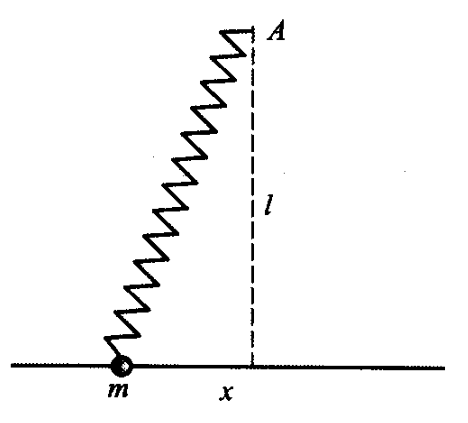
\includegraphics[width=0.31\linewidth]{figures/fig_5_3_1.png}\end{center}
\end{minipage}\par\vfill
\noindent\begin{minipage}{\textwidth}\ProblemHeading{习题}{5.4}
质量为 $m$ 的质点沿半径为 $r$ 的圆运动。弹簧一端与质点相连，另一端固定在圆外的点 $A$。点 $A$ 到圆心的距离为 $r+l$，弹簧最短时长度为 $l$，此时拉力为 $F$。求质点在该平衡位置附近微振动的角频率。
\begin{center}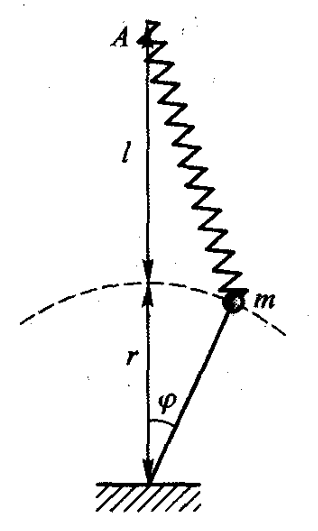
\includegraphics[width=0.18\linewidth]{figures/fig_5_4_1.png}\end{center}
\end{minipage}\par\vfill
\newpage
\noindent\begin{minipage}{\textwidth}\ProblemHeading{习题}{5.5}
在重力加速度为 $g$ 的匀强重力场中，摆球质量为 $m_2$、摆长为 $l$ 的平面单摆，其悬挂点装在质量为 $m_1$、可沿水平直线无摩擦滑动的物体上。求摆角微振动的角频率。
\begin{center}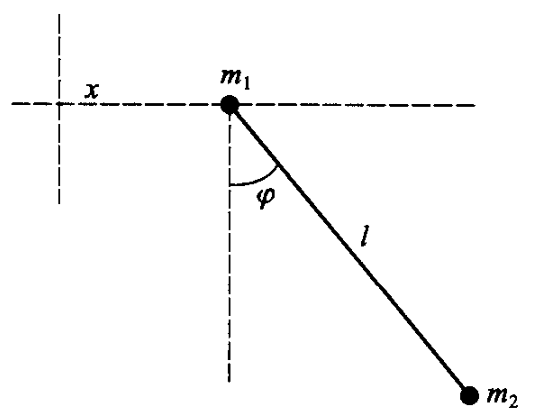
\includegraphics[width=0.24\linewidth]{figures/fig_5_5_1.png}\end{center}
\end{minipage}\par\vfill
\noindent\begin{minipage}{\textwidth}\ProblemHeading{习题}{5.6（校订）}
质点在匀强重力场中沿一条固定的光滑平面曲线运动。曲线关于经过最低点的竖直直线对称，质点绕最低点往复运动的周期与振幅无关。求曲线在该振动范围内的形状。
\end{minipage}\par\vfill
\newpage
\noindent\begin{minipage}{\textwidth}\ProblemHeading{例题}{5.7（改写）}
质量为 $m$、固有角频率为 $\omega$ 的无阻尼振子受到外力 $F(t)=f\cos(\gamma t+\beta)$。讨论下列情形。
\SubQ{1}{求 $\gamma\ne\omega$ 时的运动通解。}
\SubQ{2}{求 $\gamma=\omega$ 时的运动通解，并说明共振项的振幅随时间如何变化。}
\SubQ{3}{当 $0<|\gamma-\omega|\ll\omega$ 时，求两频率分量叠加后的振幅包络、振幅变化范围和拍频。}
\end{minipage}\par\vfill
\noindent\begin{minipage}{\textwidth}\ProblemHeading{例题}{5.8（改写）}
质量为 $m$、固有角频率为 $\omega$ 的无阻尼振子初始处在平衡位置并静止。在极短的一段时间内施加外力 $F(t)$，其作用时间远小于 $1/\omega$，总冲量为 $J=\int F(t)\,\mathrm{d}t$。求外力停止后振子的机械能在此近似下的表达式。
\end{minipage}\par\vfill
\newpage
\noindent\begin{minipage}{\textwidth}\ProblemHeading{习题}{5.9（校订）}
质量为 $m$、固有角频率为 $\omega$ 的无阻尼振子在 $t=0$ 时静止于平衡位置。对下列各外力 $F(t)$，求 $t\ge0$ 时的位移 $x(t)$。
\SubQ{1}{$F(t)=F_0$。}
\SubQ{2}{$F(t)=at$。}
\SubQ{3}{$F(t)=F_0\mathrm{e}^{-\alpha t}$。}
\end{minipage}\par\vfill
\noindent\begin{minipage}{\textwidth}\ProblemHeading{习题}{5.10（校订）}
质量为 $m$、固有角频率为 $\omega$ 的无阻尼振子在 $t=0$ 时静止于平衡位置。对下列各外力 $F(t)$，求 $t\ge0$ 时的位移 $x(t)$。
\SubQ{1}{$F(t)=F_0\mathrm{e}^{-\alpha t}\cos(\beta t)$。}
\end{minipage}\par\vfill
\newpage
\noindent\begin{minipage}{\textwidth}\ProblemHeading{习题}{5.11}
质量为 $m$、固有角频率为 $\omega$ 的无阻尼振子在 $t=0$ 时静止于未受外力时的平衡位置。外力在 $t<0$ 时为零，在 $0\le t\le T$ 时为 $F(t)=F_0t/T$，在 $t>T$ 时为 $F_0$。求 $t>T$ 时绕新的平衡位置的振幅。
\end{minipage}\par\vfill
\noindent\begin{minipage}{\textwidth}\ProblemHeading{习题}{5.12}
质量为 $m$、固有角频率为 $\omega$ 的无阻尼振子在 $t=0$ 时静止于未受外力时的平衡位置。恒力 $F_0$ 只在 $0<t<T$ 内作用，其余时刻外力为零。求 $t>T$ 时的自由振动振幅。
\end{minipage}\par\vfill
\newpage
\noindent\begin{minipage}{\textwidth}\ProblemHeading{习题}{5.13}
质量为 $m$、固有角频率为 $\omega$ 的无阻尼振子在 $t=0$ 时静止于未受外力时的平衡位置。外力只在 $0<t<T$ 内作用，在此区间内 $F(t)=F_0t/T$，其余时刻为零。求 $t>T$ 时的自由振动振幅。
\end{minipage}\par\vfill
\noindent\begin{minipage}{\textwidth}\ProblemHeading{习题}{5.14}
质量为 $m$、固有角频率为 $\omega$ 的无阻尼振子在 $t=0$ 时静止于未受外力时的平衡位置。外力仅在 $0<t<T$ 内作用，在此区间内 $F(t)=F_0\sin(\omega t)$，其中 $T=2\pi/\omega$。求 $t>T$ 时的自由振动振幅。
\end{minipage}\par\vfill
\newpage
\noindent\begin{minipage}{\textwidth}\ProblemHeading{例题}{5.15（改写）}
质量为 $m$ 的质点在三维定常势场 $U(\mathbf r)$ 的一个稳定平衡点附近运动。势能在该点的二阶导数矩阵为正定矩阵 $K$。说明如何选取简正振动的方向，并用 $K$ 的特征值表示各固有角频率。
\end{minipage}\par\vfill
\noindent\begin{minipage}{\textwidth}\ProblemHeading{习题}{5.16}
一个有两个自由度的振动系统的拉格朗日函数为
\[
L=\frac12(\dot{x}^{2}+\dot{y}^{2})-\frac{\omega_0^2}{2}(x^2+y^2)+\alpha xy.
\]
在原点为稳定平衡位置的参数范围内，求系统的简正振动和一般振动。
\end{minipage}\par\vfill
\newpage
\noindent\begin{minipage}{\textwidth}\ProblemHeading{习题}{5.17}
在重力加速度为 $g$ 的匀强重力场中，两根质量可忽略的摆杆串联在同一竖直平面内，长度分别为 $l_1,l_2$。上杆固定悬挂，上、下杆末端的质点质量分别为 $m_1,m_2$。求平面双摆在竖直向下平衡位置附近的微振动。
\begin{center}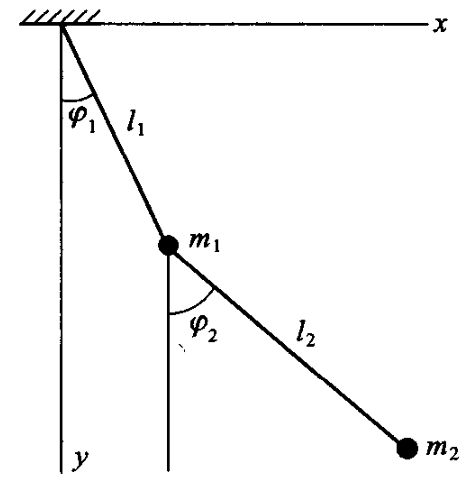
\includegraphics[width=0.24\linewidth]{figures/fig_5_17_1.png}\end{center}
\end{minipage}\par\vfill
\noindent\begin{minipage}{\textwidth}\ProblemHeading{习题}{5.18}
质量为 $m$ 的质点在有心力场 $U(r)=kr^2/2$（$k>0$）中运动，其中 $r$ 为质点到力场中心的距离。求其运动轨迹（这个系统称为空间振子）。
\end{minipage}\par\vfill
\newpage
\noindent\begin{minipage}{\textwidth}\ProblemHeading{例题}{5.19（改写）}
一个孤立分子由 $n$ 个原子组成。除去整体平动和整体转动后，求下列两种分子的各类简正振动自由度数。
\SubQ{1}{平衡构型为非共线平面构型时，分别求面内和面外的振动自由度数。}
\SubQ{2}{平衡构型为线性时，分别求纵向、横向的振动自由度数，并说明横向模式为何成对等频。}
\end{minipage}\par\vfill
\noindent\begin{minipage}{\textwidth}\ProblemHeading{习题}{5.20（校订）}
一个线性对称三原子分子 $A$--$B$--$A$ 的端原子质量为 $m_A$，中间原子质量为 $m_B$。两条键的平衡长度均为 $l$。设两键伸长量为 $\delta l_1,\delta l_2$，键角偏离平衡值的量为 $\delta$，并采用二次势能模型
\[
U=\frac{k_1}{2}\bigl[(\delta l_1)^2+(\delta l_2)^2\bigr]
  +\frac{k_2l^2}{2}\delta^2.
\]
求该分子的微振动角频率。
\begin{center}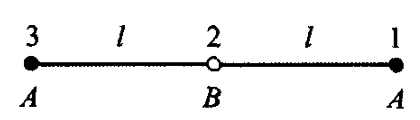
\includegraphics[width=0.25\linewidth]{figures/fig_5_20_1.png}\end{center}
\end{minipage}\par\vfill
\newpage
\noindent\begin{minipage}{\textwidth}\ProblemHeading{习题}{5.21（校订）}
一个弯曲的对称三原子分子 $A$--$B$--$A$ 的端原子质量为 $m_A$，中间原子质量为 $m_B$，平衡键角为 $2\alpha$。两条键的平衡长度均为 $l$。设两键伸长量为 $\delta l_1,\delta l_2$，键角偏离平衡值的量为 $\delta$，并采用二次势能模型
\[
U=\frac{k_1}{2}\bigl[(\delta l_1)^2+(\delta l_2)^2\bigr]
  +\frac{k_2l^2}{2}\delta^2.
\]
求该分子的微振动角频率。
\begin{center}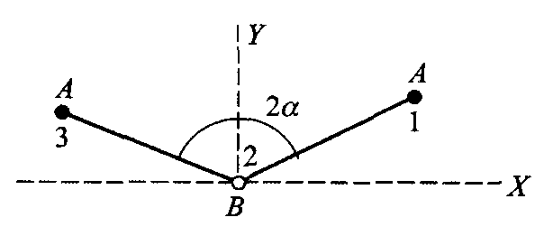
\includegraphics[width=0.3\linewidth]{figures/fig_5_21_1.png}\end{center}
\end{minipage}\par\vfill
\noindent\begin{minipage}{\textwidth}\ProblemHeading{习题}{5.22（校订）}
一个线性非对称三原子分子 $A$--$B$--$C$ 的原子质量依次为 $m_A,m_B,m_C$。$AB$、$BC$ 两键的平衡长度分别为 $l_1,l_2$，伸长量分别为 $\delta l_1,\delta l_2$。设 $\delta$ 是键角的改变量，$2l=l_1+l_2$，二次势能为
\[
U=\frac{k_1}{2}(\delta l_1)^2+\frac{k'_1}{2}(\delta l_2)^2
  +\frac{k_2l^2}{2}\delta^2.
\]
求该分子的微振动角频率。
\begin{center}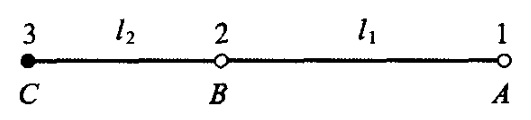
\includegraphics[width=0.31\linewidth]{figures/fig_5_22_1.png}\end{center}
\end{minipage}\par\vfill
\newpage
\noindent\begin{minipage}{\textwidth}\ProblemHeading{例题}{5.23（改写）}
质量为 $m$ 的一维振子满足 $\ddot{x}+2\lambda\dot{x}+\omega_0^2x=F(t)/m$，其中 $\lambda>0$ 为阻尼系数。设 $F(t)=f\cos(\gamma t)$。
\SubQ{1}{求稳态振幅及相位差，并在弱阻尼条件下求振幅达最大时的外力频率。}
\SubQ{2}{求弱阻尼共振附近的平均吸收功率随失谐量 $\gamma-\omega_0$ 的关系。}
\SubQ{3}{求吸收曲线的半高半宽，并说明弱阻尼近似下曲线下的面积怎样依赖阻尼系数。}
\end{minipage}\par\vfill
\noindent\begin{minipage}{\textwidth}\ProblemHeading{习题}{5.24}
质量为 $m$ 的一维振子满足 $\ddot{x}+2\lambda\dot{x}+\omega_0^2x=F(t)/m$，其中 $\lambda>0$ 为阻尼系数。取 $F(t)=f_0\mathrm{e}^{\alpha t}\cos(\gamma t)$。求由该外力产生的强迫振动分量。
\end{minipage}\par\vfill
\newpage
\noindent\begin{minipage}{\textwidth}\ProblemHeading{习题}{5.25}
无阻尼振子满足 $\ddot{x}+\omega_0^2(1+h\cos\gamma t)x=0$，其中 $0<h\ll1$。求 $\gamma=2\omega_0$ 附近参数共振的不稳定区间边界，保留至 $h^2$ 阶。
\end{minipage}\par\vfill
\noindent\begin{minipage}{\textwidth}\ProblemHeading{习题}{5.26}
无阻尼振子满足 $\ddot{x}+\omega_0^2(1+h\cos\gamma t)x=0$，其中 $0<h\ll1$。求 $\gamma=\omega_0$ 附近参数共振的不稳定区间边界的最低非零阶近似。
\end{minipage}\par\vfill
\newpage
\noindent\begin{minipage}{\textwidth}\ProblemHeading{习题}{5.27}
摆长为 $l$ 的平面单摆的悬挂点，在摆动平面内沿竖直方向按 $a\cos(\gamma t)$ 振动。设 $a\ll l$，$\gamma$ 接近 $2\sqrt{g/l}$，$g$ 为重力加速度。求摆角微振动发生参数共振的条件。
\end{minipage}\par\vfill
\noindent\begin{minipage}{\textwidth}\ProblemHeading{例题}{5.28（改写）}
弱非线性振动系统的两个一阶简正振动为 $Q_\alpha^{(1)}=a_\alpha\cos(\omega_\alpha t+\phi_\alpha)$ 和 $Q_\beta^{(1)}=a_\beta\cos(\omega_\beta t+\phi_\beta)$。某个二阶修正方程的驱动项含有乘积 $Q_\alpha^{(1)}Q_\beta^{(1)}$。求该乘积产生的频率分量和各分量的系数，并讨论两因子为同一简正振动的情形。
\end{minipage}\par\vfill
\newpage
\noindent\begin{minipage}{\textwidth}\ProblemHeading{例题}{5.29（改写）}
一个单自由度振子的运动方程为 $\ddot{x}+\omega_0^2x=-\alpha x^2-\beta x^3$。振动很弱，设基频分量为 $a\cos(\omega t)$，其中 $a$ 为小量。在逐阶近似中令较高阶修正不含基频分量。
\SubQ{1}{求 $a^2$ 阶的位移修正。}
\SubQ{2}{求基频 $\omega$ 到 $a^2$ 阶的频移，并求 $a^3$ 阶的三次谐波。}
\end{minipage}\par\vfill
\noindent\begin{minipage}{\textwidth}\ProblemHeading{例题}{5.30（改写）}
弱阻尼、弱非线性振子的运动方程为
\[
\ddot{x}+2\lambda\dot{x}+\omega_0^2x=\frac{f}{m}\cos(\gamma t)-\alpha x^2-\beta x^3.
\]
其中 $\lambda>0$、$\lambda\ll\omega_0$。记小振幅 $b$ 下非线性频移的最低阶项为 $\chi b^2$，其中 $\chi$ 为常数。设 $\gamma=\omega_0+\varepsilon$，$\lvert\varepsilon\rvert\ll\omega_0$。
\SubQ{1}{在近共振近似下，求稳态振幅 $b$ 与失谐量 $\varepsilon$ 的关系。}
\SubQ{2}{求振幅峰值，以及共振曲线首次出现多值区时的外力振幅阈值。}
\end{minipage}\par\vfill
\newpage
\noindent\begin{minipage}{\textwidth}\ProblemHeading{例题}{5.31（改写）}
弱阻尼、弱非线性振子的运动方程为
\[
\ddot{x}+2\lambda\dot{x}+\omega_0^2x=\frac{f}{m}\cos(\gamma t)-\alpha x^2-\beta x^3.
\]
其中 $\lambda>0$、$\lambda\ll\omega_0$。记小振幅 $b$ 下非线性频移的最低阶项为 $\chi b^2$，其中 $\chi$ 为常数。设 $\gamma=\omega_0/2+\varepsilon$，$\lvert\varepsilon\rvert\ll\omega_0$。求在最低非零阶近似下产生的近共振驱动项，并求频率为 $2\gamma$ 的振动分量的稳态振幅与失谐量 $\varepsilon$ 的关系。
\end{minipage}\par\vfill
\noindent\begin{minipage}{\textwidth}\ProblemHeading{例题}{5.32（改写）}
弱阻尼、弱非线性振子的运动方程为
\[
\ddot{x}+2\lambda\dot{x}+\omega_0^2x=\frac{f}{m}\cos(\gamma t)-\alpha x^2-\beta x^3.
\]
其中 $\lambda>0$、$\lambda\ll\omega_0$。记小振幅 $b$ 下非线性频移的最低阶项为 $\chi b^2$，其中 $\chi$ 为常数。设 $\gamma=2\omega_0+\varepsilon$，$\lvert\varepsilon\rvert\ll\omega_0$。
\SubQ{1}{求频率为 $\gamma/2$ 的小扰动所满足的线性化方程，并确定它发生参数型共振的条件。}
\SubQ{2}{计入最低阶非线性频移，求频率为 $\gamma/2$ 的稳态共振分量的可能振幅。}
\end{minipage}\par\vfill
\newpage
\noindent\begin{minipage}{\textwidth}\ProblemHeading{习题}{5.33}
弱阻尼、弱非线性振子的运动方程为
\[
\ddot{x}+2\lambda\dot{x}+\omega_0^2x=\frac{f}{m}\cos(\gamma t)-\alpha x^2-\beta x^3.
\]
其中 $\lambda>0$、$\lambda\ll\omega_0$。记小振幅 $b$ 下非线性频移的最低阶项为 $\chi b^2$，其中 $\chi$ 为常数。设 $\gamma=3\omega_0+\varepsilon$，$\lvert\varepsilon\rvert\ll\omega_0$。求在最低非零阶近似下，频率为 $\gamma/3$ 的共振分量的稳态振幅 $b$ 与失谐量 $\varepsilon$ 的关系。
\end{minipage}\par\vfill
\noindent\begin{minipage}{\textwidth}\ProblemHeading{习题}{5.34}
在重力加速度为 $g$ 的匀强重力场中，摆长为 $l$ 的平面单摆的悬挂点在摆动平面内沿竖直方向按 $a\cos(\gamma t)$ 作高频振动，其中 $\gamma\gg\sqrt{g/l}$，且 $a\ll l$。求快振动平均后的摆角的稳定平衡位置及其存在条件。
\end{minipage}\par\vfill
\newpage
\noindent\begin{minipage}{\textwidth}\ProblemHeading{习题}{5.35}
在重力加速度为 $g$ 的匀强重力场中，摆长为 $l$ 的平面单摆的悬挂点在摆动平面内沿水平方向按 $a\cos(\gamma t)$ 作高频振动，其中 $\gamma\gg\sqrt{g/l}$，且 $a\ll l$。求快振动平均后的摆角的稳定平衡位置及其存在条件。
\end{minipage}\par\vfill
